\documentclass[10pt,openright,twoside,french]{book}

\usepackage{marvosym}
\input philippe2013
\input philippe2013_activites

\usepackage{docmute}

\pagestyle{empty}

\begin{document}
\renewcommand\MaCouleur{Purple}

%___________________________
%===    Page de garde
%------------------------------------------------------

\frontmatter

\input{1sti2d_Page_Titre_Activites}

\pieddepage{}{}{}
\entete{}{}{}

\mainmatter

\entete{}{{\color{\MaCouleur} \textbullet~\leftmark~\textbullet}}{}
\pieddepage{}{\color{\MaCouleur}$\stackrel{***}{\thepage}$}{}

%------ Chapitre 01 - Statistiques
    %------------------ Activité 1
        \documentclass[10pt,openright,twoside,french]{book}
\input philippe2013
\input philippe2013_activites
\pagestyle{empty}

\begin{document}

\TitreActivite{i.1}{Calculer une moyenne\par Faire le bon choix}

On s'intéresse à la distance entre des établissements scolaires publics et la piscine utilisée par chacun d'entre eux.\par
Une étude du ministère de l'\'Education Nationale a déterminé que cette distance était, au moment de l'étude :
\begin{itemize}
    \item comprise entre $0{,}2~km$ et $1{,}5~km$ dans huit régions ;
    \item supérieure à $1{,}5~km$ et au plus égale à $2{,}5~km$ dans onze régions ;
    \item supérieure à $2{,}5~km$ dans trois régions.
\end{itemize}\medskip

\begin{enumerate}
    \item Considérons neuf lycées notées $A$, $B$,\ldots, $I$ dont la distance à la piscine correspondante est donnée dans le tableau suivant :
    \begin{center}
    \renewcommand\arraystretch{1.5}
        \begin{tabular}{|c|>\centering p{1.75em}|>\centering p{1.75em}|>\centering p{1.75em}|>\centering p{1.75em}|>\centering p{1.75em}|%
        >\centering p{1.75em}|>\centering p{1.75em}|>\centering p{1.75em}| p{1.75em}|}
            \hline
            Lycée & $A$ & $B$ & $C$ & $D$ & $E$ & $F$ & $G$ & $H$ & \multicolumn{1}{c|}{$I$} \\
            \hline
            Distance en km & $1{,}8$ & $1{,}0$ & $20{,}2$ & $0$ & $0{,}6$ & $0$ & $0{,}8$ & $2{,}6$ & $0$\\
            \hline
        \end{tabular}
    \end{center}
    
    Pour cet ensemble de neuf lycées, calculer la distance moyenne à la piscine fréquentée. Dans laquelle des trois catégories définies ci-dessus doit-on classer cet ensemble de neuf lycées ?\medskip
    
    \item Les neuf lycées ont les effectifs suivants :
    \begin{center}
    \renewcommand\arraystretch{1.5}
        \begin{tabular}{|c|>\centering p{2.5em}|>\centering p{2.5em}|>\centering p{2.5em}|>\centering p{2.5em}|>\centering p{2.5em}|%
        >\centering p{2.5em}|>\centering p{2.5em}|>\centering p{2.5em}| p{2.5em}|}
            \hline
            Lycée & $A$ & $B$ & $C$ & $D$ & $E$ & $F$ & $G$ & $H$ & \multicolumn{1}{c|}{$I$} \\
            \hline
            Effectifs & $930$ & $\NP{1130}$ & $\NP{420}$ & $\NP{1710}$ & $\NP{1450}$ & $\NP{1430}$ & $\NP{1920}$ & $\NP{530}$ & $\NP{1250}$\\
            \hline
        \end{tabular}
    \end{center}
    
    Calculer la distance moyenne par élève parcourue pour se rendre à la piscine (les informations du premier tableau doivent être utilisées).\medskip
    
    \item Afin de calculer les frais de déplacements entre les lycées et les piscines, laquelle des deux distances moyennes paraît la plus appropriée ?
\end{enumerate}


\end{document} \clearpage
    %------------------ Activité 2
        \input{01_Act02_Indicateurs_Position}\clearpage
    %------------------ Activité 3
        \input{01_Act03_Indicateurs_Dispersion}\clearpage

%------ Chapitre 02 - Etudes de fonctions
    %------------------ Activité 1
        \documentclass[10pt,openright,twoside,french]{book}
\input philippe2013
\input philippe2013_activites
\pagestyle{empty}


\begin{document}

\TitreActivite{ii.1}{Modéliser des mesures}

À l'aide d'un ohmmètre, un ingénieur fait la mesure de la résistance $R$ aux bornes d'un radiateur électrique pour chacune des positions du bouton de commande (10 puissances possibles). Le tableau des valeurs de résistances (en ohms, arrondies à l'entier près) pour les différentes valeurs de puissances $P$ est donné ci-dessous.

\begin{center}
    \begin{tabular}{|>\bfseries c|*{10}{c|}}
        \hline
            Position bouton & 1 & 2 & 3 & 4 & 5 & 6 &7 & 8 & 9 & 10 \\
        \hline
            $P$ (en watts) & $200$ & $400$ & $600$ & $800$ & $\np{1000}$ & $\np{1200}$ & $\np{1400}$ & $\np{1600}$ & $\np{1800}$ & $\np{2000}$ \\
        \hline
            $R$ (en ohms) & $264$ & $132$ & $88$ & $66$ & $53$ & $44$ & $38$ & $33$ & $29$ & $26$ \\
        \hline
            \rule{0cm}{20pt} & & & & & & & & & & \\
        \hline
    \end{tabular}
\end{center}

\begin{enumerate}
    \item Dans le repère \Oij ci-dessous, placer les points de coordonnées $(P \pv R)$ pour chacun des couples donnés dans le tableau ($1~cm$ pour $200~W$ en abscisses et $1~cm$ pour $20~\Omega$ en ordonnées).
    \item Relier les points précédents pour représenter l'allure de la courbe représentative de la fonction qui à $P$ fait correspondre $R$.
    \item Cette courbe a la même allure que quelle autre courbe de fonction vue en seconde ? Quelle est le nom de ce type de courbe ?
    \item Dans la ligne vide du tableau, calculer pour chaque valeur $\sqrt{P \times R}$. Arrondir à l'unité près.
    \item Déduire une expression de $R$ en fonction de $P$ le plus possible en accord avec les résultats obtenus.
    \item Déterminer alors la valeur de résistance que devrait présenter le radiateur pour fournir une puissance de chauffe de $\np{3000}~W$.
\end{enumerate}
\begin{center}
    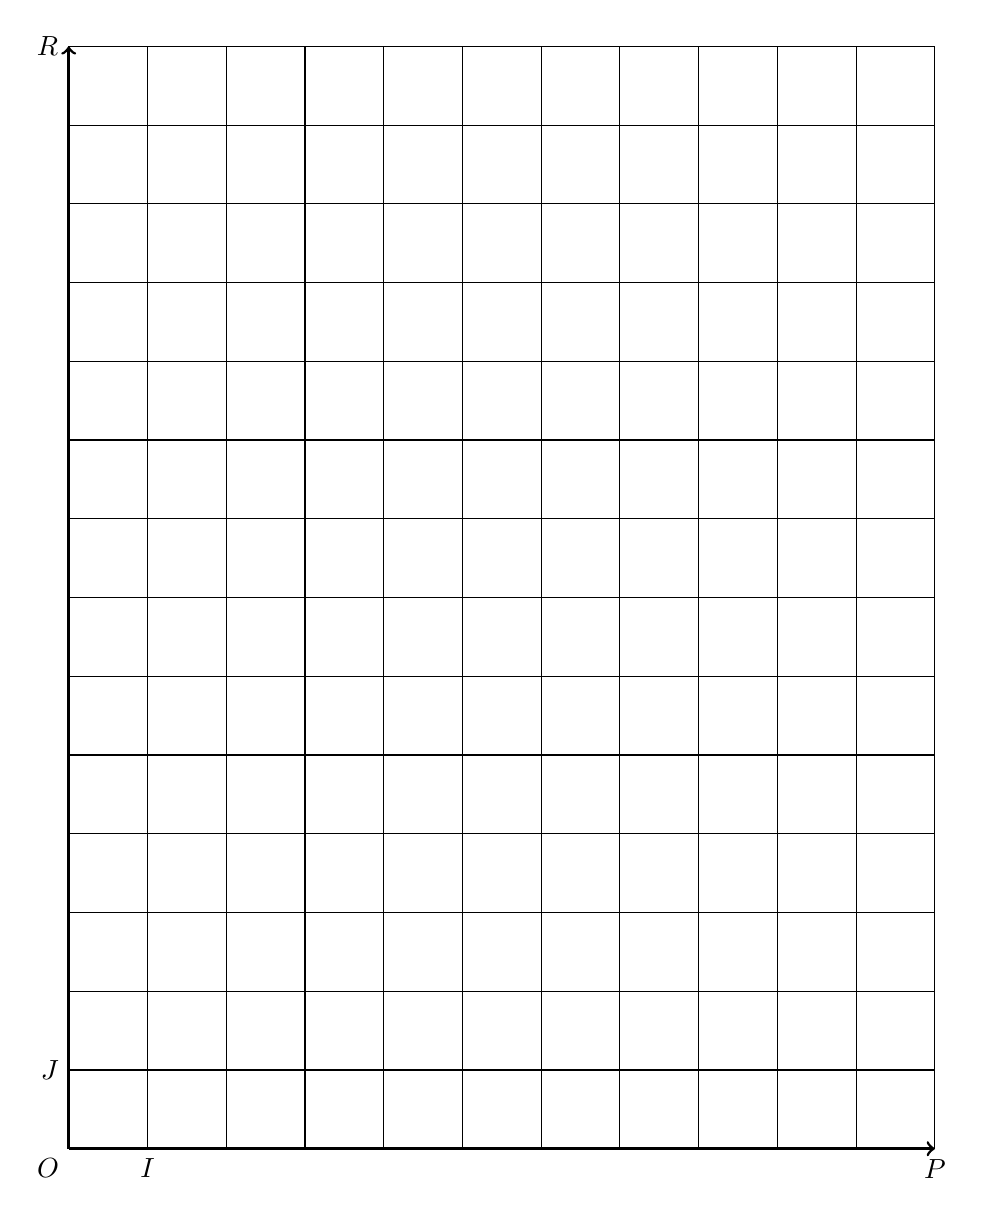
\begin{tikzpicture}[x=1cm,y=1cm]
        \draw[line width = 0.4pt] (0,0) grid[xstep=1,ystep=1] (11,14);
        \draw[line width = 1pt,->] (0,0) -- (11,0) node[below] {$P$};
        \draw[line width = 1pt,->] (0,0) -- (0,14) node [left] {$R$};
        \coordinate (O) at (0,0); \draw (O) node[below left] {$O$};
        \coordinate (I) at (1,0); \draw (I) node[below] {$I$};
        \coordinate (J) at (0,1); \draw (J) node[left] {$J$};
    \end{tikzpicture}
\end{center}


\end{document} \clearpage
    %------------------ Activité 2
        \documentclass[10pt,openright,twoside,french]{book}
\input philippe2013
\input philippe2013_activites
\pagestyle{empty}


\begin{document}

\TitreActivite{ii.2}{Fonction valeur absolue}

On appelle \textbf{valeur absolue} d'un nombre réel $x$ le nombre \textbf{positif}, noté $\abs x$, défini par :
\[\abs x =
\left\{\begin{array}{r@{ \text{ si } }l}
	x & x \geq 0 \\
	-x & x \leq 0
\end{array}\right.\]

\begin{enumerate}
	\item À combien est égale $\abs{12}$ ? Et $\abs{-12}$ ?
	\item Compléter le tableau suivant :\medskip

{
	\footnotesize
		\renewcommand{\arraystretch}{1.5}
		\begin{tabular}{|c|*{13}{>{\scriptsize\centering\arraybackslash}m{0.65cm}|}}
			\hline
				$x$ & $-3$ & $-2,5$ & $-2$ & $-1,5$ & $-1$ & $-0,5$ & $0$ & $0,5$ & $1$ & $1,5$ & $2$ & $2,5$ & $3$ \\
			\hline
				$\abs x$ &&&&&&&&&&&&& \\
			\hline
		\end{tabular}
}\medskip

\item Sur le repère ci-dessous, représenter la fonction $v \colon x \mapsto \abs x$.

\begin{center}
    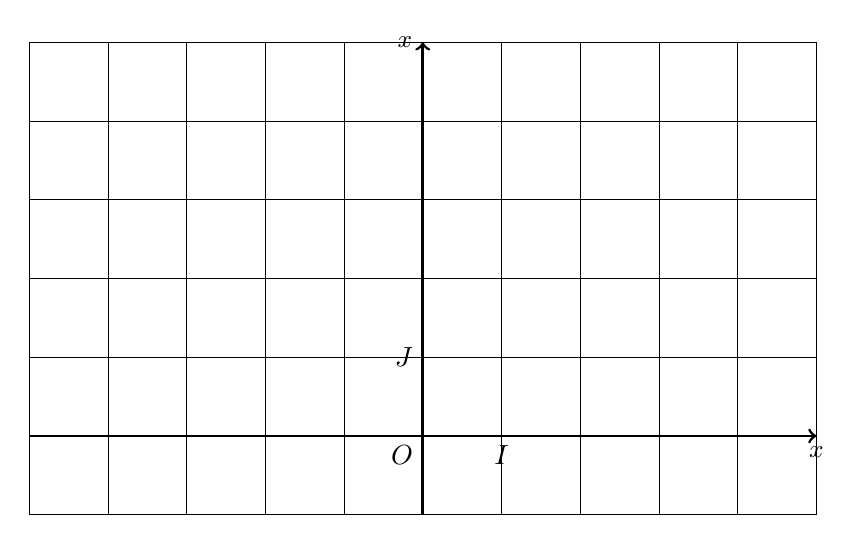
\begin{tikzpicture}[x=1cm,y=1cm]
        \draw[line width = 0.2pt] (-5,-1) grid[xstep=1,ystep=1] (5,5);
        \draw[line width = 1pt,->] (-5,0) -- (5,0) node[below] {\small $x$};
        \draw[line width = 1pt,->] (0,-1) -- (0,5) node [left] {\small $\abs x$};
        \coordinate (O) at (0,0); \draw (O) node[below left] {$O$};
        \coordinate (I) at (1,0); \draw (I) node[below] {$I$};
        \coordinate (J) at (0,1); \draw (J) node[left] {$J$};
    \end{tikzpicture}
\end{center}

\item Dessiner le tableau de variation de la fonction $v$ puis déterminer le minimum de $v$.
\item Sur l'intervalle $\intervalleof{-\infty}{0}$, la fonction $v$ coïncide avec quelle autre fonction ?
\item Même question sur l'intervalle $\intervallefo{0}{+\infty}$.
\end{enumerate}

\end{document} \clearpage
    %------------------ Activité 3
        \documentclass[10pt,openright,twoside,french]{book}
\input philippe2013
\input philippe2013_activites
\pagestyle{empty}


\begin{document}

\TitreActivite{ii.3}{Représentation graphique \par de fonctions composées}

Le plan est muni du repère orthonormal \Oij. On définit la fonction $u$ sur l'intervalle $\intervalleff{-2}{4}$ dont on donne la représentation graphique $\calig C$ ci-dessous.

\begin{center}
	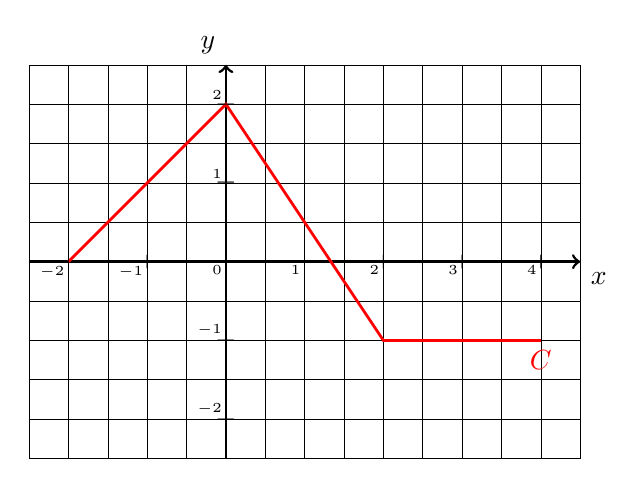
\begin{tikzpicture}
		\draw[line width = 0.2pt] (-2.5,-2.5) grid[xstep=0.5,ystep=0.5] (4.5,2.5);
		\draw[line width = 1pt,->] (-2.5,0)--(4.5,0) node[below right] {$x$};
		\draw[line width = 1pt,->] (0,-2.5)--(0,2.5) node[above left] {$y$};
		\draw[line width=1pt,color=red] (-2,0) -- (0,2) -- (2,-1) -- (4,-1) node[below] {$\calig C$};
		\foreach \x in {-2,-1,...,4} \draw(\x,0) node {\tiny$\vert$} node[below left=-2pt] {\tiny $\x$};
		\foreach \x in {-2,-1} \draw(0,\x) node {$-$} node[above left=-2pt] {\tiny $\x$};
		\foreach \x in {2,1} \draw(0,\x) node {$-$} node[above left=-2pt] {\tiny $\x$};
	\end{tikzpicture}
\end{center}

\section*{Fonction $u + k$}
\begin{enumerate}
	\item Compléter le tableau suivant :
	\begin{center}
		\renewcommand{\arraystretch}{1.5}
		\begin{tabular}{|c|*{7}{>{\centering\arraybackslash}m{1cm}|}}
			\hline
				$x$ & $-2$ & $-1$ & $0$ & $1$ & $2$ & $3$ & $4$ \\
			\hline
				$u(x)$ & & & & & & & \\
			\hline
				$f(x) = u(x) + 1$ & & & & & & & \\
			\hline
				$g(x) = u(x) - 2$ & & & & & & & \\
			\hline
		\end{tabular}
	\end{center}
	\item Sur le repère ci-dessous, construire \textbf{en rouge} la courbe $\calig C_1$ représentative de $f$ et \textbf{en vert} la courbe $\calig C_2$ représentative de $g$.
	\item Indiquer comment obtenir $\calig C_1$ et $\calig C_2$ en fonction de $\calig C$.
\end{enumerate}\medskip

\begin{center}
	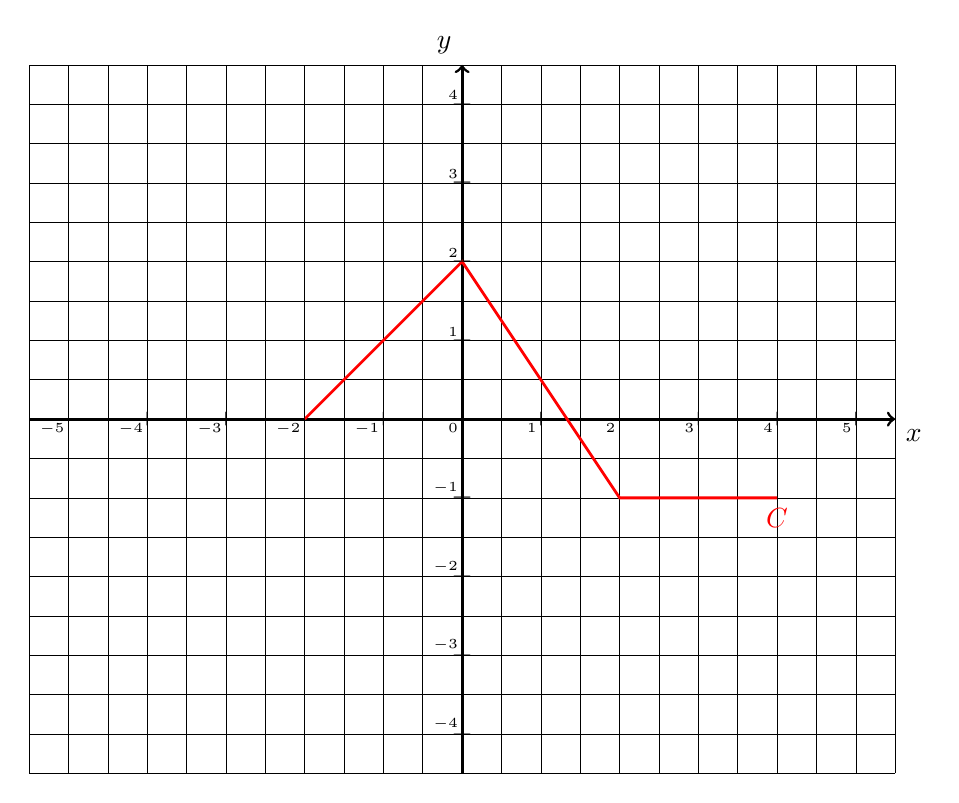
\begin{tikzpicture}
		\draw[line width = 0.2pt] (-5.5,-4.5) grid[xstep=0.5,ystep=0.5] (5.5,4.5);
		\draw[line width = 1pt,->] (-5.5,0)--(5.5,0) node[below right] {$x$};
		\draw[line width = 1pt,->] (0,-4.5)--(0,4.5) node[above left] {$y$};
		\draw[line width=1pt,color=red] (-2,0) -- (0,2) -- (2,-1) -- (4,-1) node[below] {$\calig C$};
		\foreach \x in {-5,-4,...,5} \draw(\x,0) node {\tiny$\vert$} node[below left=-2pt] {\tiny $\x$};
		\foreach \x in {-4,-3,...,-1} \draw(0,\x) node {$-$} node[above left=-2pt] {\tiny $\x$};
		\foreach \x in {1,2,...,4} \draw(0,\x) node {$-$} node[above left=-2pt] {\tiny $\x$};
	\end{tikzpicture}
\end{center}

\section*{Fonction $t \mapsto u(t + \lambda)$}

\begin{enumerate}
	\item Sur le repère ci-dessous, construire en vert la courbe $\calig C_3$ obtenue par une translation \textbf{horizontale} de tous les points de $\calig C$ d'une unité \textbf{vers la gauche}.
	\item On appelle $h$ la fonction dont la représentation graphique est $\calig C_3$.
	\begin{enumerate}
		\item Sur quel intervalle $I_1$ la fonction $h$ est-elle définie ?
		\item Pour les valeurs entières de $I_1$, a-t-on $h(t) = u(t + 1)$ ou $h(t) = u(t - 1)$ ?
	\end{enumerate}
	\item Toujours sur le repère ci-dessous, construire en bleu la courbe $\calig C_4$ obtenue par une translation \textbf{horizontale} de tous les points de $\calig C$ de deux unités \textbf{vers la droite}.
	\item On appelle $\ell$ la fonction dont la représentation graphique est $\calig C_4$.
	\begin{enumerate}
		\item Sur quel intervalle $I_2$ la fonction $\ell$ est-elle définie ?
		\item Pour les valeurs entières de $I_2$, a-t-on $\ell(t) = u(t + 2)$ ou $\ell(t) = u(t - 2)$ ?
	\end{enumerate}
\end{enumerate}

\begin{center}
	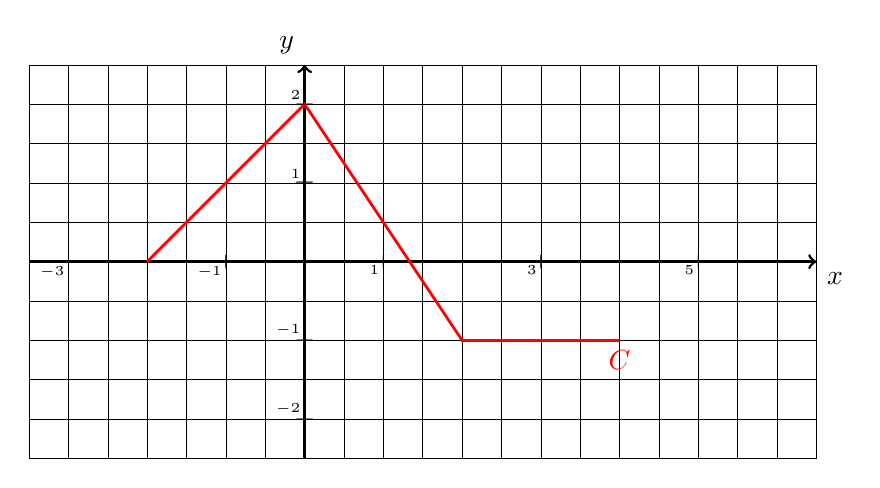
\begin{tikzpicture}
		\draw[line width = 0.2pt] (-3.5,-2.5) grid[xstep=0.5,ystep=0.5] (6.5,2.5);
		\draw[line width = 1pt,->] (-3.5,0)--(6.5,0) node[below right] {$x$};
		\draw[line width = 1pt,->] (0,-2.5)--(0,2.5) node[above left] {$y$};
		\draw[line width=1pt,color=red] (-2,0) -- (0,2) -- (2,-1) -- (4,-1) node[below] {$\calig C$};
		\foreach \x in {-3,-1,...,6} \draw(\x,0) node {\tiny$\vert$} node[below left=-2pt] {\tiny $\x$};
		\foreach \x in {-2,-1} \draw(0,\x) node {$-$} node[above left=-2pt] {\tiny $\x$};
		\foreach \x in {2,1} \draw(0,\x) node {$-$} node[above left=-2pt] {\tiny $\x$};
	\end{tikzpicture}
\end{center}

\section*{Fonction $\abs u$}
\begin{enumerate}
	\item Compléter le tableau suivant :
	\begin{center}
		\renewcommand{\arraystretch}{1.5}
		\begin{tabular}{|c|*{7}{>{\centering\arraybackslash}m{1cm}|}}
			\hline
				$x$ & $-2$ & $-1$ & $0$ & $1$ & $2$ & $3$ & $4$ \\
			\hline
				$u(x)$ & & & & & & & \\
			\hline
				$m(x) = \abs{u(x)}$ & & & & & & & \\
			\hline
		\end{tabular}
	\end{center}
	\item Sur le repère ci-dessous, construire \textbf{en rouge} la courbe $\calig C_5$ représentative de $m$.
	\item Quel est le signe de $m$ ?
\end{enumerate}\medskip

\begin{center}
	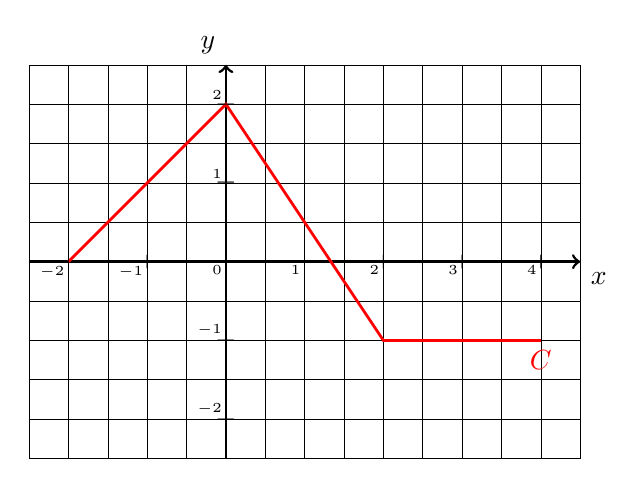
\begin{tikzpicture}
		\draw[line width = 0.2pt] (-2.5,-2.5) grid[xstep=0.5,ystep=0.5] (4.5,2.5);
		\draw[line width = 1pt,->] (-2.5,0)--(4.5,0) node[below right] {$x$};
		\draw[line width = 1pt,->] (0,-2.5)--(0,2.5) node[above left] {$y$};
		\draw[line width=1pt,color=red] (-2,0) -- (0,2) -- (2,-1) -- (4,-1) node[below] {$\calig C$};
		\foreach \x in {-2,-1,...,4} \draw(\x,0) node {\tiny$\vert$} node[below left=-2pt] {\tiny $\x$};
		\foreach \x in {-2,-1} \draw(0,\x) node {$-$} node[above left=-2pt] {\tiny $\x$};
		\foreach \x in {2,1} \draw(0,\x) node {$-$} node[above left=-2pt] {\tiny $\x$};
	\end{tikzpicture}
\end{center}

\end{document} \clearpage
        
%------ Chapitre 03 - Cercle trigonométrique
    %------------------ Activité 1
        \documentclass[10pt,openright,twoside,french]{book}
\input preambule_2013

\newcommand\TitreActivite[2]{%
    \setcounter{exo}{0}
        \begin{center}
            \psframebox[shadow=true,shadowcolor=gray!75,shadowsize=3pt,%
            framearc=0.3,%
            fillstyle=gradient,gradmidpoint=0.8,gradangle=20,gradbegin=red!60!yellow!40,gradend= white]{%
                \parbox{0.5\linewidth}{%
                    \begin{center}
                        \Large\bfseries
                        \uuline{Activité \bsc{#1}}\par
                        #2
                    \end{center}}}
        \end{center}\bigskip
}

\pagestyle{empty}


\begin{document}

\TitreActivite{iii.1}{Cosinus et Sinus \par Cercle trigonométrique}

\exo Pour chaque question :
\begin{itemize}
    \item Faire une figure à main levée ;
    \item Répondre à la question sans utiliser le théorème de Pythagore ;
    \item Arrondir les résultats au centième près.
\end{itemize}

\begin{enumerate}
    \item Soit $ABC$ un triangle rectangle en $B$ tel que $AB = \SI{5}{cm}$ et $\widehat{BAC} = \ang{25}$.\par
    Calculer les longueurs $AC$ et $BC$.
    \item Soit $DEF$ un triangle rectangle en $D$ tel que $DF = \SI{8,5}{cm}$ et $\widehat{DEF} = \ang{75}$.\par
    Calculer les longueurs $DE$ et $EF$.
    \item Soit $GHI$ un triangle rectangle en $I$ tel que $GH = \SI{5}{cm}$, $HI = \SI{12}{cm}$ et $GI = \SI{13}{cm}$.\par
    Calculer la mesure de chacun des angles du triangle.
\end{enumerate}\medskip

\exo
On se place dans un repère \Oij avec $4$ carreaux comme unité de longueur. $I$ est le point de coordonnées $(1 \pv 0)$.

\begin{enumerate}
    \item Réaliser la figure suivante :
    \begin{enumerate}
        \item Dessiner le repère et le cercle trigonométrique $\calig U$ ;
        \item Placer le point $M$ sur $\calig U$ tel que $IOM = \ang{45}$ ;
        \item Placer le point $H$, projeté orthogonal de $M$ sur l'axe des abscisses ;
        \item Placer le point $K$, projeté orthogonal de $M$ sur l'axe des ordonnées.
    \end{enumerate}
    \item
    \begin{enumerate}
        \item Le triangle $OMH$ est-il rectangle ? Pourquoi ? Quel côté est l'hypoténuse ? Quelle est sa longueur ?
        \item Donner l'expression de $\cos\left(\widehat{IOM}\right)$ en fonction d'un des côtés du triangle $OMH$.
        \item À l'aide de la calculatrice, déterminer alors l'abscisse du point $M$.
        \item Le triangle $OMK$ est-il rectangle ? Pourquoi ? Quel côté est l'hypoténuse ? Quelle est sa longueur ?
        \item Donner l'expression de $\sin\left(\widehat{KMO}\right)$ en fonction d'un des côtés du triangle $OMK$.
        \item Expliquer pourquoi $\widehat{KMO} = \widehat{IOM}$ et donner alors l'expression de $\sin\left(\widehat{IOM}\right)$ en fonction d'un des côtés du triangle $OMK$.
        \item À l'aide de la calculatrice, déterminer alors l'ordonnée du point $M$.
    \end{enumerate}
    \item
    \begin{enumerate}
        \item Placer le point $N$ sur $\calig U$ tel que $ION =  \rad{\dfrac\pi3}$.
        \item Lire les coordonnées du point $N$. En déduire alors les valeurs de $\cos\left(\dfrac\pi3\right)$ et $\sin\left(\dfrac\pi3\right)$.
        \item Vérifier à la calculatrice.
    \end{enumerate}
    \item
    \begin{enumerate}
        \item Déterminer graphiquement les valeurs exactes de $\cos\left(-\dfrac\pi3\right)$ et $\sin\left(-\dfrac\pi3\right)$.
        \item Déterminer graphiquement les valeurs exactes de $\cos\left(\dfrac{2\pi}{3}\right)$ et $\sin\left(\dfrac{2\pi}{3}\right)$.
    \end{enumerate}
    \item On place un point $P$ sur le cercle $\calig U$ tel que $\widehat{IOP} = \rad\alpha$.
    \begin{enumerate}
        \item Graphiquement, comment déterminer $\cos(\alpha)$ et $\sin(\alpha)$ ?
        \item Où placer le point $P$ pour avoir $\cos(\alpha) > 0$ et $\sin(\alpha) < 0$ ?
        \item Où placer le point $P$ pour avoir $\cos(\alpha) < 0$ et $\sin(\alpha) < 0$ ?
        \item Où placer le point $P$ pour avoir $\cos(\alpha) = 0$ ?
        \item Où placer le point $P$ pour avoir $\sin(\alpha) = 0$ ?
    \end{enumerate}
\end{enumerate}

\end{document} 

\clearpage
\strut
\pieddepage{}{}{}
\entete{}{}{}
\vspace{\stretch{1}}

\[***\]

\begin{center}
\'Ecrit par Philippe \bsc{De Sousa}.\par
Dernière modification le \today.
\end{center}

\end{document} 